\documentclass[12pt, a4paper, twoside]{article}
\usepackage[utf8]{inputenc}
\usepackage[spanish]{babel}
\usepackage{hyperref}
\usepackage{fancyhdr}
\usepackage{graphicx}
\usepackage{enumitem}

\pagestyle{fancy}
\fancyhf{}
\fancyfoot[R]{\thepage}
\fancyfoot[L]{\nouppercase{\leftmark}}
\fancyhead[R]{Resumen C\&C en IS.}
\fancyhead[L]{Carlos G. Pérez Aranda. }


\graphicspath{{./images/}}
\title{Resumen de la asignatura Cognición y Comunicación en Ingeniería del Software}


\begin{document}
\maketitle

\section{hasta el 04/03/2025}


\section{Clase del 04 de marzo.}
Tenemos 4 exposiciones según la imagen adjunta:
\begin{figure}[h]
    \centering
    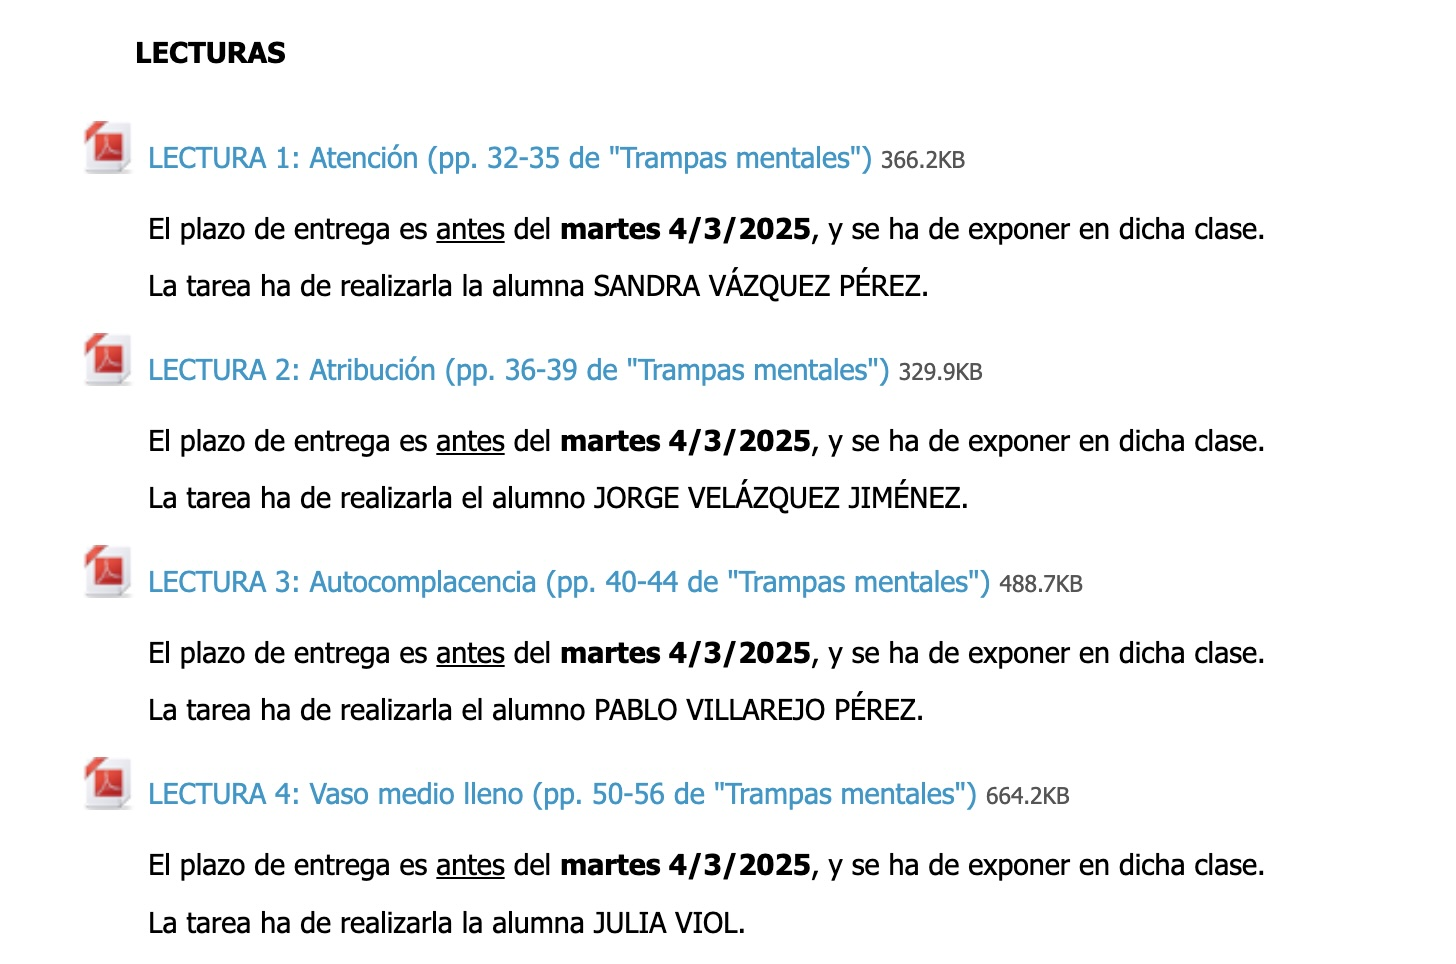
\includegraphics[width=0.9\textwidth]{./images/0304.jpg}
    \caption{lecturas del día}
\end{figure}

\subsection{Exposición 1 - Trampas mentales}
Como nuestra mente nos engaña. \\
\begin{itemize}
\item{La falta de atención nos hace no ver fallos y cosas obvias, ejemplo Pulp Fiction y sus
errores de continuidad. }
\item{Bloopers.it dedicada a los errores de las películas. }
\item{Encuentra las 5 diferencias, cambios en el campo visual que no percibimos. Explicación 
fisiológica (parpadeos, movimientos oculares, etc). }
\item{El Club de la Lucha y sus fotogramas pornográficos de los que la mayoría de las personas
no de percatan.}
\end{itemize}
Aplicación en la ingeniería del software:
\begin{itemize}
\item{Errores de programación}
\item {errores de configuración}
\item {errores de seguridad}
\item {errores de rendimiento}
\item {...otros}
\end{itemize}



\subsection{Exposición 2 - Como nos vemos a nosotros mismos en comparación a los demás}
Historia del águila criada con pollos
\begin{itemize}
    \item{Atribución Disposicional: Explicamos el comportamiento de los demás basándonos en su personalidad}
    \item {Atribución Situacional: Explicamos nuestro comportamiento basándonos en la situación}
\end{itemize}
Jones  y Nisbett identificaron que juzamos de manera diferente si somos actores o espectadores..

\begin{itemize}
    \item{Error en el código como falta de habilidad}
    \item{No siempre se considera la presión de los factores externos}
    \item {Puede conllevar baja moral en el equipo.}
\end{itemize}

Kepler estimó 13 días para calcular la órbita de Marte, pero le llevó años.\\

Fomentar factres situacionales, mejorar la comunicación para evitar atribuciones injustas,
fomentar la empatía y la comprensión.\\

\subsection{Exposición 3 - Autocomplacencia}

La satisfacción por los propios actos o por la propia condición o manera de ser.\\
Conversación entre Aristipo y Platón.\\
Somos muy sensibles a los vicios de los demás y ciegos a los propios como mecanismo
de defensa del ego. \\
\begin{itemize}
    \item{En los éxitos: Soy el mejor.}
    \item{En los fracasos: No es mi culpa, tuve mala suerte.}
\end{itemize}
%% poner en negrita
\textbf{Experimento sobre ansiedad y autocomplacencia:} 

\begin{itemize}
    \item{Bug -> La culpa es del lenguaje.}
    \item{Tiempo -> El cliente cambió los requisitos.}
    \item{Equipo -> No entienden mi código.}
\end{itemize}

\noindent\textbf{Solución:}

\begin{itemize}
    \item{Feedback honesto.}
    \item{Métricas objetivas.}
    \item{Análisis post morten.}
    \item{Primer paso para la mejora es aceptarlo.}
\end{itemize}

\subsection{Lectura 4 - Vaso medio lleno}
Poco que señalar aquí, la presentación fue en inglés, pero aunque entiendo el idioma la 
compañera habló muy bajito y no se escuchaba nada.\\

\subsection{Resumen}
\begin{itemize}
    \item El fondo negro no es adecuado para los proyectores y clases.
    \item Hay que presentarse. Soy fulano de tal y os voy a hablar de ...
    \item El tamaño de letra en el límite.
    \item Hay que moverse por el atril.
    \item Si se hace mención a un vídeo es una oportunidad magnífica para ponerlo.
    \item Poner imágenes en las presentaciones.
    \item Lenguaje no verbal, las manos no en los bolsillos ni cruzados de brazos.
    \item El puntero es un buen apoyo.
    
\end{itemize}

\newpage

\section{Clase del 05 de marzo}

Tenemos 4 exposiciones más según la imagen adjunta:
\begin{figure}[h]
    \centering
    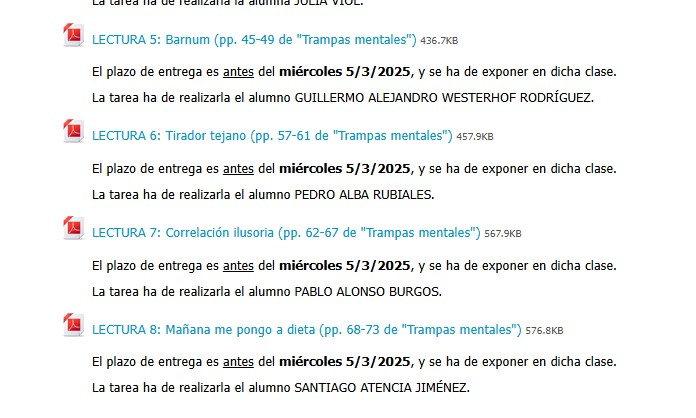
\includegraphics[width=0.9\textwidth]{./images/0305.jpg}
    \caption{lecturas del día}
\end{figure}

\subsection{Barnum}
Descripción del efecto Barnum y cómo las declaraciones generales pueden parecer personales y precisas.

Falacia de la validación personal.

\subsection{Wishful thinking}
Considerar que algo es más probable o cierto porque se desea que así sea. Este sesgo puede llevar a la toma de decisiones irracionales y a la sobreestimación de las probabilidades de éxito.

\begin{itemize}
    \item{Ejemplo en ingeniería del software: Creer que un proyecto se completará a tiempo a pesar de las señales de advertencia.}
    \item{Solución: Realizar evaluaciones objetivas y basadas en datos.}
\end{itemize}

L'oreal, porque tú lo vales.\\

Test de personalidad "Brain works". El efecto Forer y cómo las personas pueden identificarse con descripciones generales, es másw pronunciado en 
personas con trantornos psicóticos, en especial la desorganización cognitiva.

\textbf{Myers-Brigs Type Indicator}, test de personalidad basado en la teoría de Jung. muy usado para
reclutamiento de software y tests de personalidad.\\

\subsection{Tirador Lejano}
Explicación del sesgo del tirador lejano y cómo se pueden encontrar patrones significativos en datos aleatorios.
\begin{itemize}
    \item Experimento de la moneda. Tirar 4 veces la moneda de 4 en 4 
    \item Exámenes tipo test. Cómo va a salir dos veces seguidas la respuesta b, mucho menos 3 veces.
    \item Incidencia del cancer infantil en una zona por encima de lo normal. Se echa la culpa a factores ambientales.
\end{itemize}

El Tirador Tejano.\\

Realiza un tiro y luego pinta el blanco. Dando a entender que es un tirador infalible.

\begin{itemize}
    \item Métricas engañosas
    \item Sesgo en validación de datos
    \item Ajuste de requisitos.
    \item Gestión de proyectos, informes de progreso en áreas cn problemas críticos.
    \item Machiune learning. Entrenar un modelo con unos datos que luego se usen para ver la correlación de las predicciones.
\end{itemize}

Solución:

\begin{itemize}
    \item Definir métricas relevantes.
    \item Pruebas rigurosas.
    \item Evitar la manipulación de los requisitos
    \item Revisión de los datos.
    \item Validación cruzada.
\end{itemize}

Tomar decisiones basadas en evidencia real, tener en cuenta la objetividad y el engaño puede llevar a decisiones equivocadas costosas.

\subsection{Correlación ilusoria}
Discusión sobre la correlación ilusoria y cómo las personas pueden percibir relaciones entre eventos que no existen.

Zanahoria y la vista. Es totalmente falso la correlación etre comer zanahorias y tener buena vista. Lo mismo pasa con los 
amuletos, relacionamos dos hechos independientes.

Debe evitarse decir algo como espero que lo hayan entendido, porque puede llevar a que los oyentes sientan que se les está llamando tontos.


\subsection{Mañana me pongo a dieta}
Reflexión sobre la procrastinación y la tendencia a posponer tareas importantes.

¿Por qué no cumplimos los propósitos de año nuevo?

Pagar para no ir al gimnasio. Mañana será más fácil. Beneficio futuro. 
Coste inmediato para un beneficio futuro.

Cuando queremos hacer algo para el futuro solemos postergarlo. La falacia de la planificación. 
Cuanto tiempo estima un alumno que va a tardar en hacer una tesis, 33.9 días de media. solamente el 30\%
de los alumnos lo terminan en ese tiempo.

Ley Hofstader: Todo lleva más tiempo del que crees, incluso si tienes en cuenta la Ley de Hofstader.

Personas retardatorias, siempre dejan todo para el último momento.

Genera tanto estrés iniciar una tarea que les cuesta mucho empezarla.

\subsection{Conclusiones}

No decir 'Me ha tocado tal...'.


No decir 'Espero que lo hayan entendido'

Poner transparencia final.

Está bien ponerse como ejemplo de algo, da cercanía.

Poner conclusiones.

\newpage

\section{Clase del 10 de marzo}

Tenemos 4 exposiciones según la imagen adjunta:

\begin{figure}[h]
    \centering
    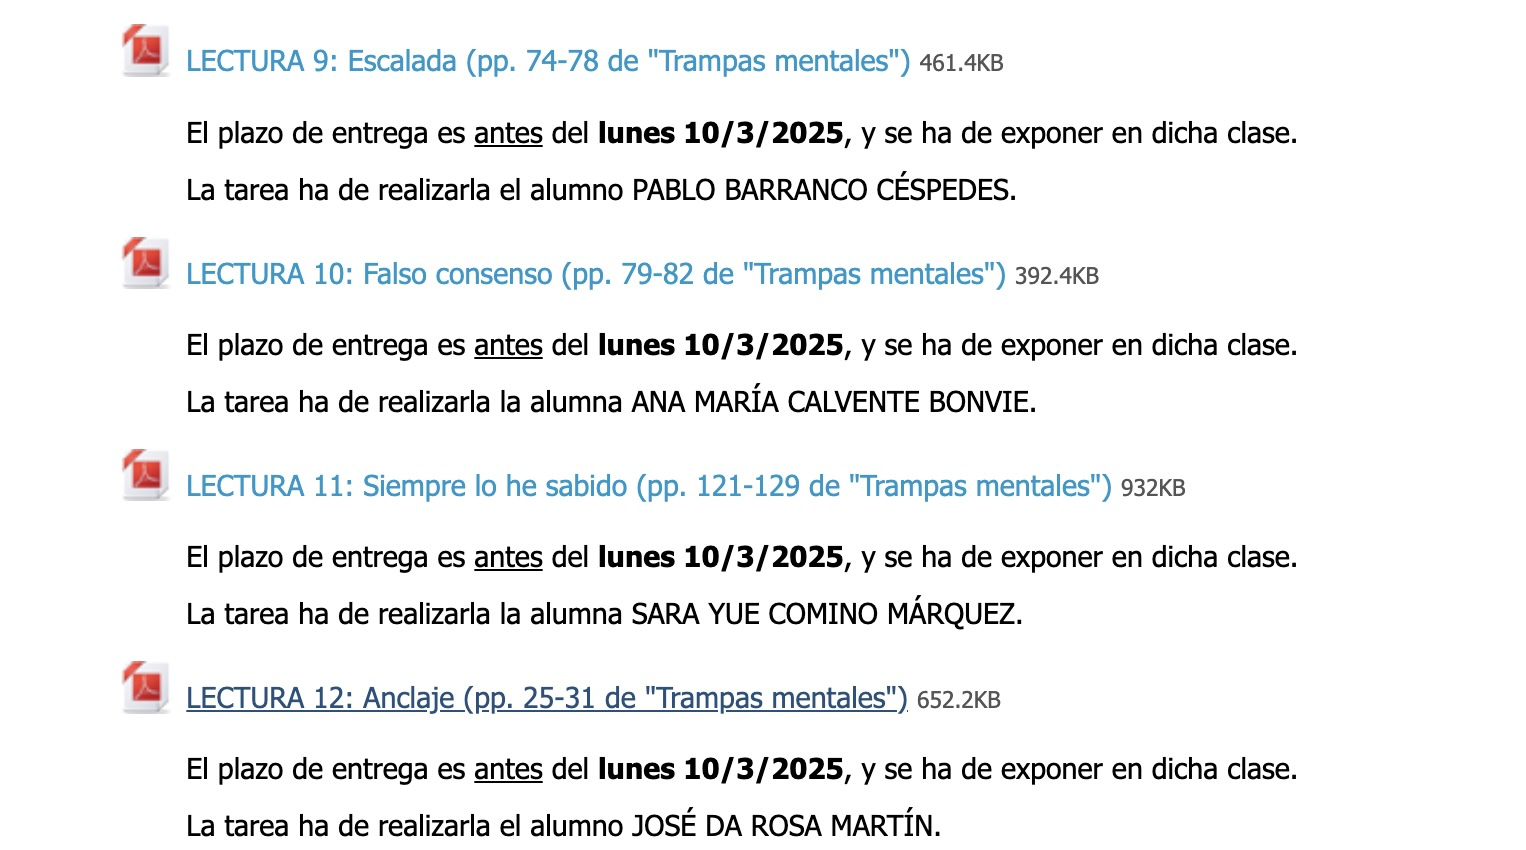
\includegraphics[width=0.9\textwidth]{./images/0310.jpg}
    \caption{lecturas del día}
\end{figure}

\subsection{Escalada}

Descripción de la escalada de compromiso y cómo las personas pueden continuar invirtiendo en una decisión a pesar de que los resultados sean negativos.

¿Gastaríamos el dinero más a gusto si pudiéramos elegir dónde estamos?

Pone el ejemplo de jugar en un campo de fútbol. Ya que hemos pagado nos quedamos con nuestra elección
aunque no sea la mejor.

Lubik - Experimento de la subasta. Se subasta un billete de 20 euros. La persona que gana la subasta
paga 20 euros y se lleva el billete. La persona que pierde la subasta paga lo que ha pujado y no se lleva nada.

Los que caen en este tipo de juegos son débiles a este efecto.

El Proyecto concorde se pone de ejemplo de este efecto ya que se invirtieron muchos millones en él durante
toda su vida útil.  


Soluciones:

\begin{itemize}
    \item No entrar al juego.
    \item Si entras, tener un plan de salida y ejecutarlo lo antes posible.

\end{itemize}

\newpage
En Desarrollo de Software:
\begin{itemize}
    \item No seguir invirtiendo en un proyecto que no tiene futuro.
    \item No seguir invirtiendo en un proyecto que no tiene futuro.
    \item No seguir invirtiendo en un proyecto que no tiene futuro.
    \item Desarrollo de sw vs costes hundidos
    \item Decisiones de mantenimiento vs reescritura de sw.
    \item Metodologías ágiles y gestión del cambio.
    \item Compra de sw y herramientas.
\end{itemize}


\subsection{Falso Consenso}

Discusión sobre el falso consenso y cómo las personas pueden sobreestimar la cantidad de personas que comparten sus opiniones o creencias.
¿Por qué todos se parecen a mi?.

Lee Ross en los 70. La gente tiende a pensar que los demás piensan como ellos.
Experimento del "Hombre Anuncio" en el que se pide a los participantes que lleven un cartel de "No a la violencia" y se les pregunta si creen que los demás también llevarán el cartel. La mayoría piensa que sí.
Entre los que aceptaron llevar el cartel, la mayoría pensaba que los demás también lo harían.
Entre los que no aceptaron llevar el cartel, la mayoría pensaba que los demás tampoco lo harían.

Si nosotros elegimos algo pensamos que la mayoría de las personas también lo harían.

Richar Thaler al principio del milenio, escribió un artículo en el Journal of Economics Perspectives en el que hablaba de la economía conductual. En él hablaba de la falacia del falso consenso.
En el que se preguntaba si el sujeto tenía móvil y si pensaba que los demás también lo tenían con resultados análogos al experimento anterior.  

Cuando estamos solos nos fiamos mñas de nuestro propio criterio.

Bernard Whitley - experimento con 260 estudiantes femeninas no casadas.



\subsection{Siempre lo he sabido}

Reflexión sobre la profecía autocumplida y cómo las expectativas pueden influir en el comportamiento y los resultados.


Profetas del día después.

Se hizo un estudio a 160 médicos divididos en dos grupos a los que se les presentó un caso, a uno de los grupos se les dio el diagnóstico
y al otro no. El grupo que tenía el diagnóstico previo tuvo la percepción mayoritaria de que ese era el diagnóstico que hubieran dado, el grupo 
al que no se le facilitó el diagnóstico no tuvo esa percepción (sólo el 30\%).
\\\

Aplicaciones en la ingeniería del software:
\begin{itemize}
    \item Post-morten analysis.
    \item Estimación de costes y tiempos.
    \item Toma de decisiones técnicas.
    \item Análisis de bugs y fallos.
    \item Aprendizaje de proyectos fallidos.
\end{itemize}


\subsection{Anclaje}
Explicación del sesgo de anclaje y cómo las personas pueden depender demasiado de la información inicial al tomar decisiones.\\
\textit{Se aplaza para otro día}


\subsection{\textit{Conclusiones}}
\begin{itemize}
    \item En la diapositiva final poner el nombre de la presentación.
    \item Cuidado con el tamaño de letra.
    \item Si se ponen experimentos, poner los años.
    \item Pocas transparencias en Siempre lo he sabido (sólo 12 transparencias, las otras 15 y 18).

\end{itemize}

\section{Clase del 18 de marzo}

Tenemos 4 exposiciones de las lecturas de la siguiente imagen
\begin{figure}[h]
    \centering
    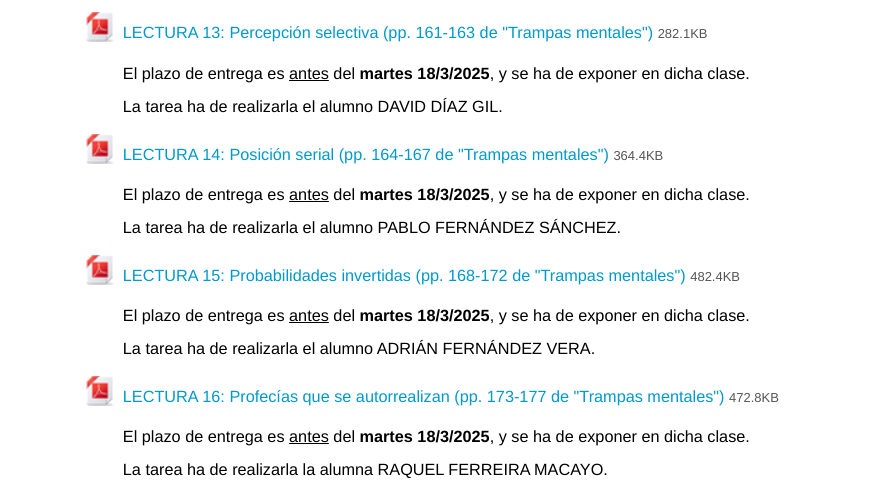
\includegraphics[width=0.9\textwidth]{./images/0318.png}
    \caption{lecturas del día}
\end{figure}
\subsecion{Percepción Selectiva}
Validación basada en expextativas.\\
Sesgo en interpretación de bugs.\\
Falsa seguridad en cuanto a la seguridad del software.\\
Programación de errores difíciles de detectar hasta que es demasiado tarde.\\.
Daños reputacionales.\\
\subsecion{Posición serial}
\subsection{}
\subsection{Profecías Autorealizadas}
Efecto placebo.\\
Definición del efecto placebo.\\
El oráculo de matrix.\\
\subsection{Conclusiones}




\end{document}